\chapter{Gráficos de resultados de la evaluación}
\label{cap:gre}

En el presente anexo se revisan algunos ejemplos de los gráficos obtenidos del análisis.

\section{Gráficos sin normalizar para una sola imagen}

\begin{figure}[H]
  \centering
  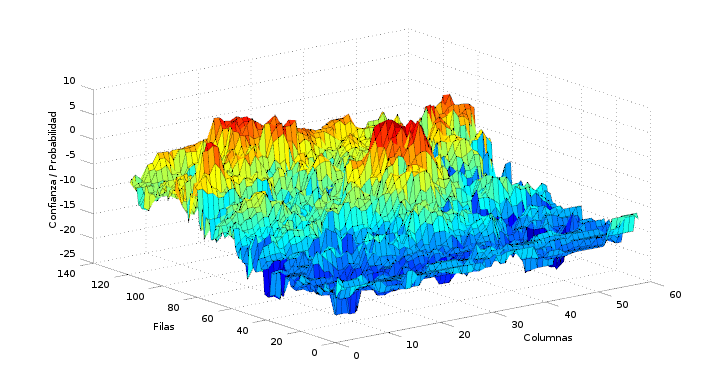
\includegraphics[scale=.6]{images/raw/boost/prueba2}
  \caption{\em  Resultados ``crudos'' obtenidos de la detección de una sola imagen utilizando una ventana de clasificación de 32x64px. Obtenido de la combinación descriptor/clasificador HOG/Adaboost.}  
  \label{fig:gsn1}
\end{figure}

\begin{figure}[H]
  \centering
  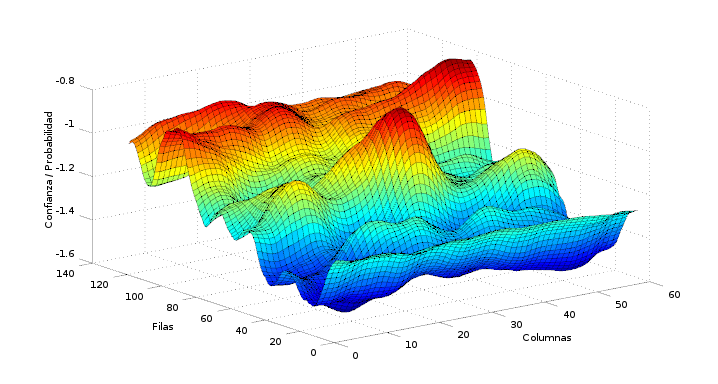
\includegraphics[scale=.6]{images/raw/svm/prueba2}
  \caption{\em  Resultados ``crudos'' obtenidos de la detección de una sola imagen utilizando una ventana de clasificación de 32x64px. Obtenido con la combinación descriptor/clasificador HOG/SVM lineal.}  
  \label{fig:gsn2}
\end{figure}

 
\section{Gráficos normalizados para una sola imagen}

\begin{figure}[H]
  \centering
  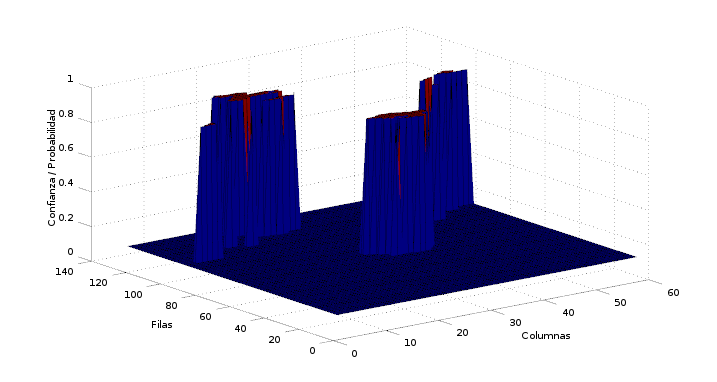
\includegraphics[scale=.6]{images/sig/boost/prueba2}
  \caption{\em  Resultados probabilísticos obtenidos de la detección de una sola imagen utilizando una ventana de clasificación de 32x64px. Obtenido de la combinación descriptor/clasificador HOG/Adaboost.}  
  \label{fig:gn1}
\end{figure}

\begin{figure}[H]
  \centering
  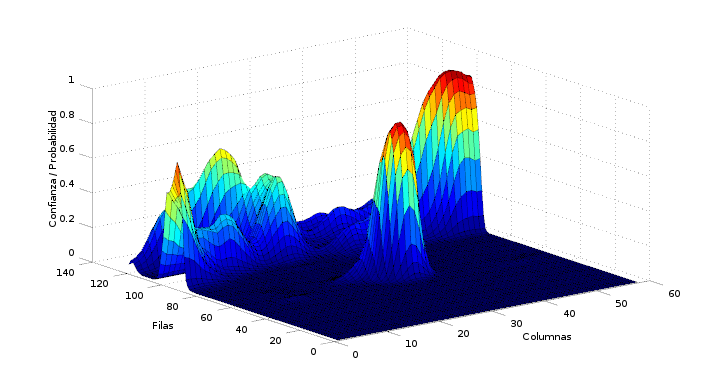
\includegraphics[scale=.6]{images/sig/svm/prueba2}
  \caption{\em  Resultados probabilísticos obtenidos de la detección de una sola imagen utilizando una ventana de clasificación de 32x64px. Obtenido con la combinación descriptor/clasificador HOG/SVM lineal.}  
  \label{fig:gn2}
\end{figure}


\section{Gráficos de promedio de repuesta normalizada}


\begin{figure}[H]
  \centering
  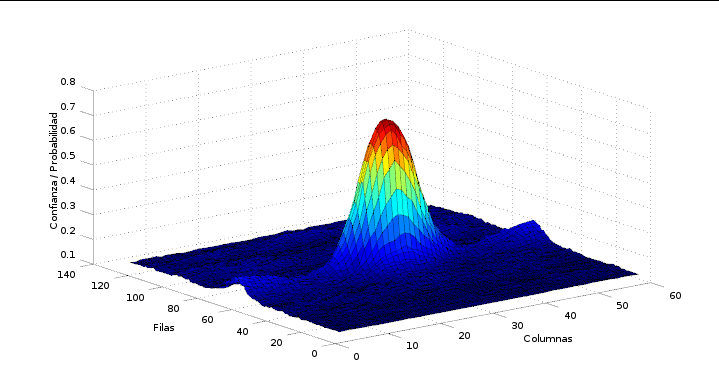
\includegraphics[scale=.6]{images/mean/boost/32}
  \caption{\em  Resultados promedio de la detección de todas las imágenes del set de datos utilizando una ventana de clasificación de 32x64px. Obtenido de la combinación descriptor/clasificador HOG/Adaboost.}  
  \label{fig:gp1}
\end{figure}

\begin{figure}[H]
  \centering
  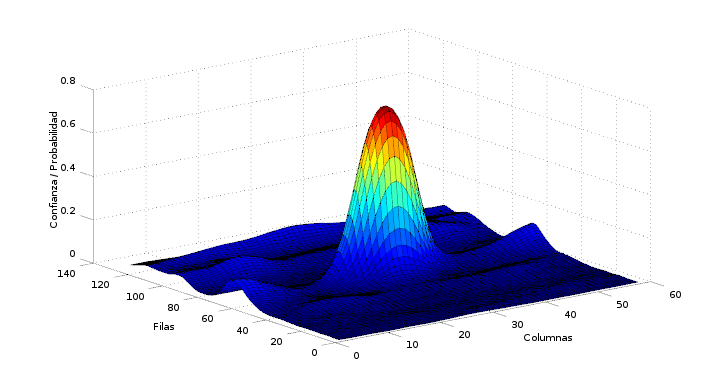
\includegraphics[scale=.6]{images/mean/svm/32}
  \caption{\em  Resultados promedio de la detección de todas las imágenes del set de datos utilizando una ventana de clasificación de 32x64px. Obtenido con la combinación descriptor/clasificador HOG/SVM lineal.}  
  \label{fig:gp2}
\end{figure}

\begin{figure}[H]
  \centering
  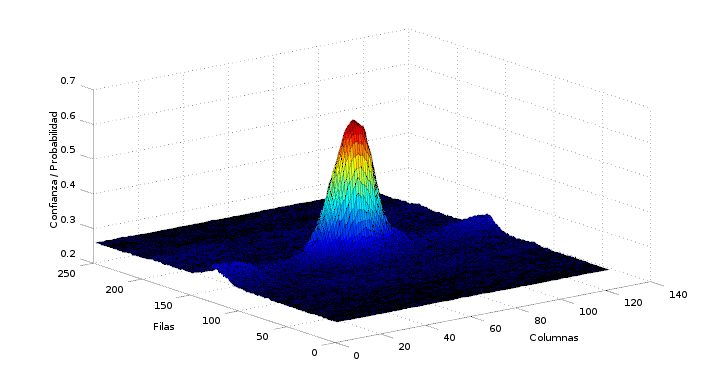
\includegraphics[scale=.6]{images/mean/boost/64}
  \caption{\em  Resultados promedio de la detección de todas las imágenes del set de datos utilizando una ventana de clasificación de 64x128px. Obtenido de la combinación descriptor/clasificador HOG/Adaboost.}  
  \label{fig:gp3}
\end{figure}

\begin{figure}[H]
  \centering
  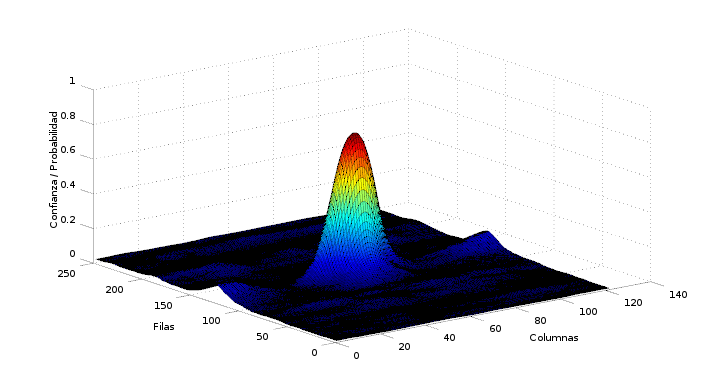
\includegraphics[scale=.6]{images/mean/svm/64}
  \caption{\em  Resultados promedio de la detección de todas las imágenes del set de datos utilizando una ventana de clasificación de 64x128px. Obtenido con la combinación descriptor/clasificador HOG/SVM lineal.}  
  \label{fig:gp4}
\end{figure}

\begin{figure}[H]
  \centering
  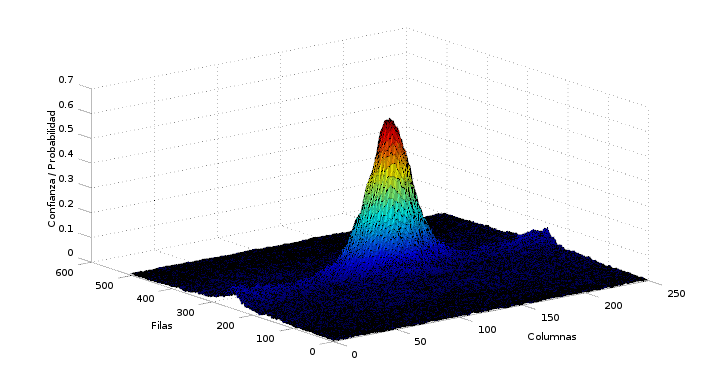
\includegraphics[scale=.6]{images/mean/boost/128}
  \caption{\em  Resultados promedio de la detección de todas las imágenes del set de datos utilizando una ventana de clasificación de 128x256px. Obtenido de la combinación descriptor/clasificador HOG/Adaboost.}  
  \label{fig:gp5}
\end{figure}

\begin{figure}[H]
  \centering
  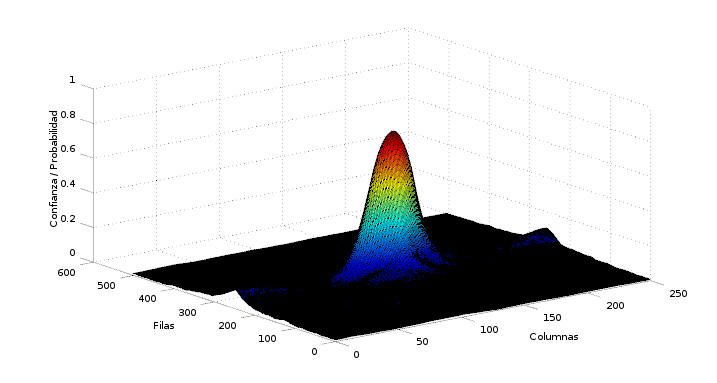
\includegraphics[scale=.6]{images/mean/svm/128}
  \caption{\em  Resultados promedio de la detección de todas las imágenes del set de datos utilizando una ventana de clasificación de 128x256px. Obtenido con la combinación descriptor/clasificador HOG/SVM lineal.}  
  \label{fig:gp6}
\end{figure}

\begin{figure}[H]
  \centering
  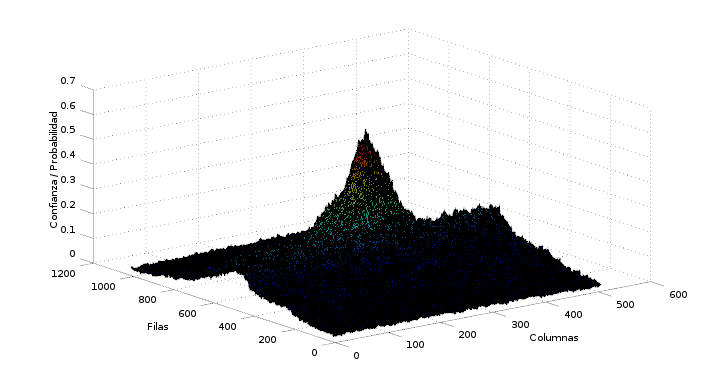
\includegraphics[scale=.6]{images/mean/boost/256}
  \caption{\em  Resultados promedio de la detección de todas las imágenes del set de datos utilizando una ventana de clasificación de 256x512px. Obtenido de la combinación descriptor/clasificador HOG/Adaboost.}  
  \label{fig:gp7}
\end{figure}

\begin{figure}[H]
  \centering
  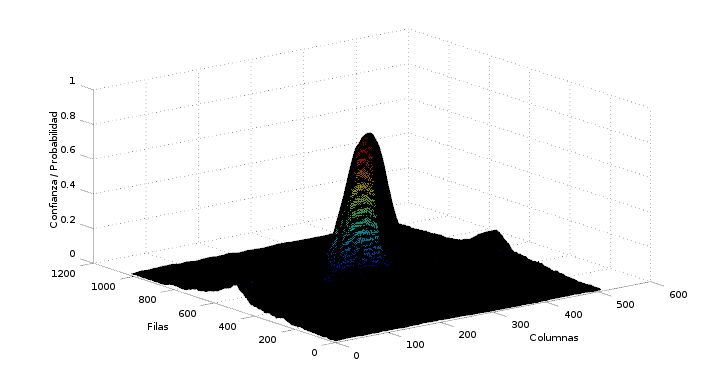
\includegraphics[scale=.6]{images/mean/svm/256}
  \caption{\em  Resultados promedio de la detección de todas las imágenes del set de datos utilizando una ventana de clasificación de 256x512px. Obtenido con la combinación descriptor/clasificador HOG/SVM lineal.}  
  \label{fig:gp8}
\end{figure}


\section{Gráficos completos de evaluación PPD}

\begin{figure}[H]
  \centering
  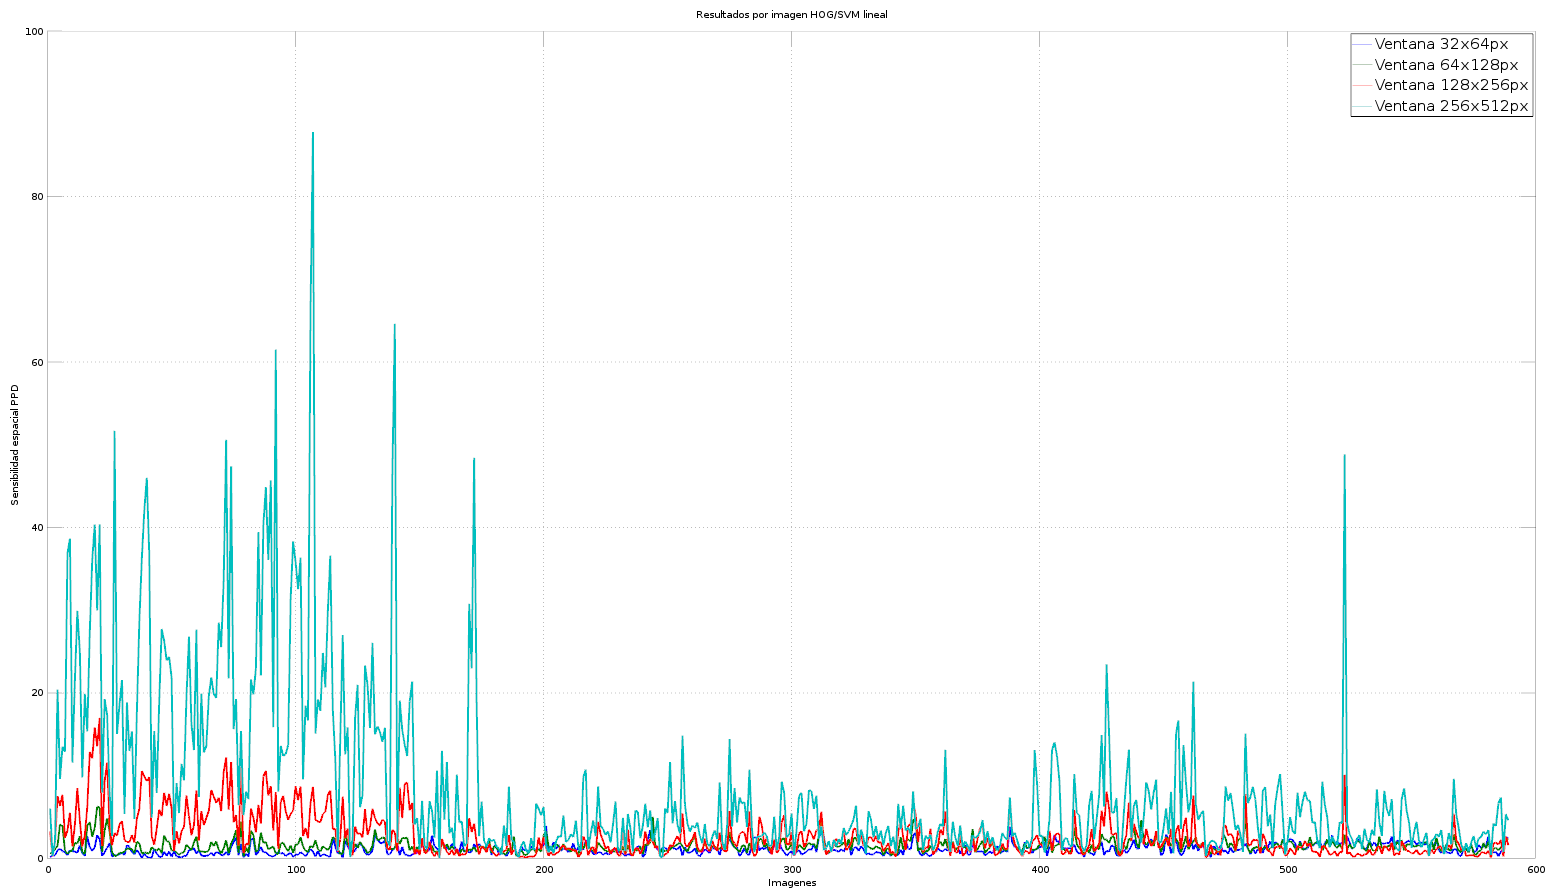
\includegraphics[scale=.25]{images/fullresultssvm}
  \caption{\em  Resultado de la evaluación de PPD para cada imagen en el set de datos en cada una de las escalas utilizando HOG/SVM lineal.}  
  \label{fig:gcsvm}
\end{figure}

\begin{figure}[H]
  \centering
  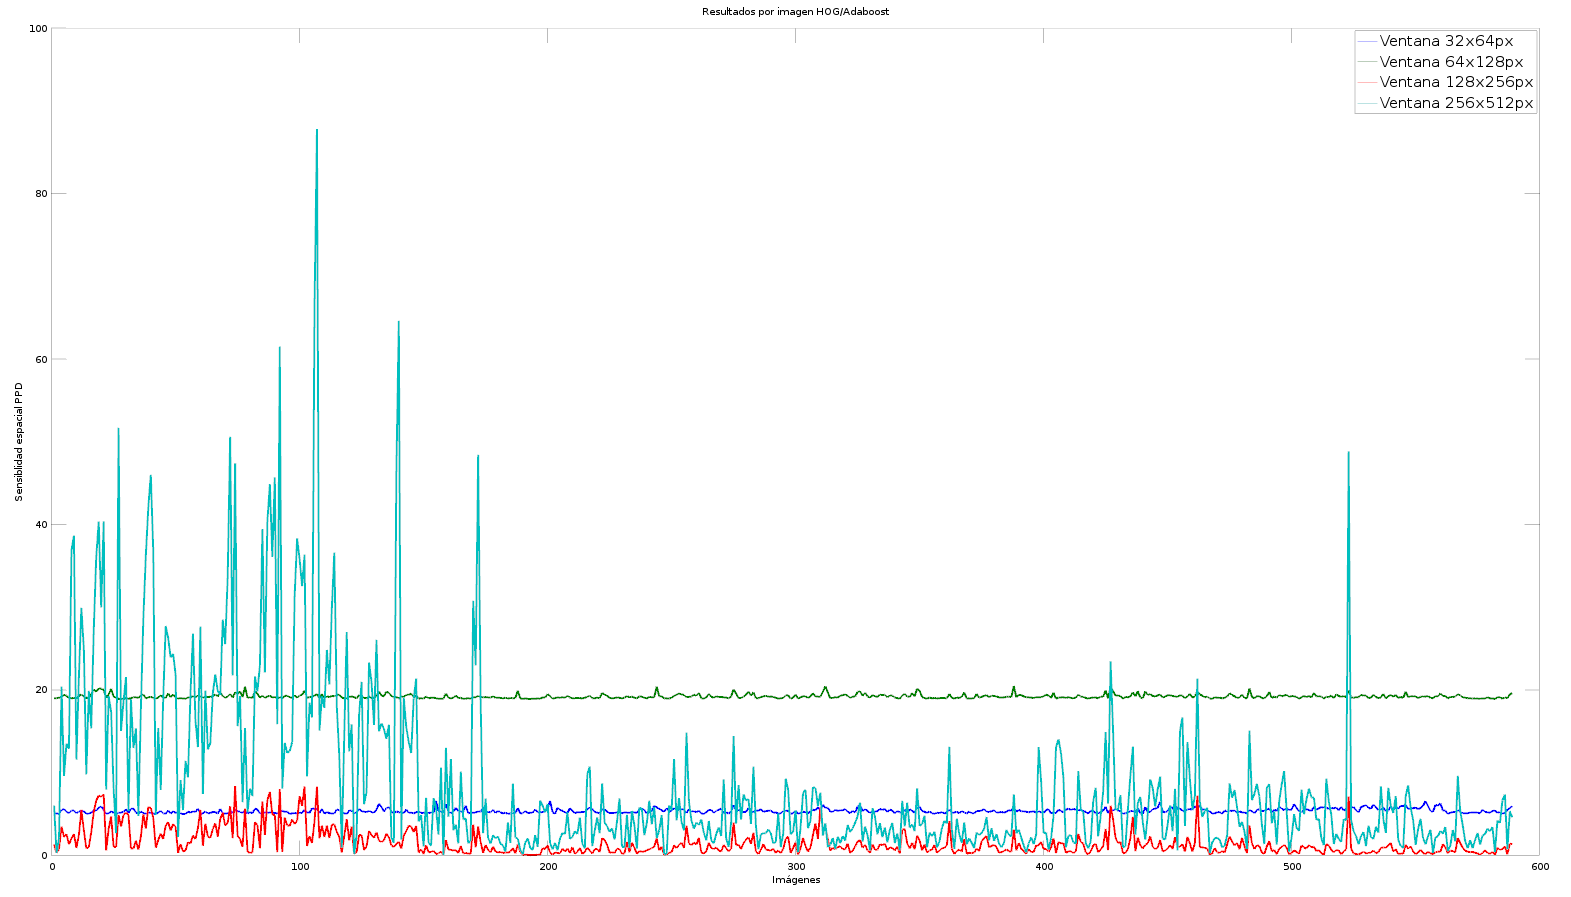
\includegraphics[scale=.25]{images/fullresultsboost}
  \caption{\em  Resultado de la evaluación de PPD para cada imagen en el set de datos en cada una de las escalas utilizando HOG/Adaboost.}  
  \label{fig:gcboost}
\end{figure}
